\documentclass[12pt, oneside]{article} 
\usepackage[left=15mm, right=15mm, top=10mm]{geometry}
\usepackage{graphicx}
\usepackage{url}
\usepackage{multicol}
\usepackage{lipsum}
\usepackage{mwe}
\usepackage{float}

\begin{document}
\title{Techniques d'attaque - chiffrement RSA}
\author{Tristan BILOT, Nora DELFAU, Enzar SALEMI, Madushan THAMBITHURAI\\EPITA}
\date{31 Mai 2021}
\maketitle

\begin{abstract}
Vous travaillez dans le département de criminologie informatique du département de surveillance des cyber-territoires. Les services secrets ont intercepté un message chiffré (texte chiffré) envoyé par une personne (sous surveillance) à son ami. Le message a été chiffré à l'aide de l'algorithme de chiffrement symétrique AES-256-CBC. La clé avec laquelle ce message a été chiffré a été dérivée d'un mot de passe envoyé chiffré par l'algorithme de chiffrement asymétrique RSA. Vous devez casser la clé et trouver le message initial (texte brut). Selon les premières informations dont vous disposez, l'outil qui a été utilisé pour générer la paire de clés asymétriques a été mal configuré. Par conséquent, la qualité des nombres premiers choisis était médiocre. Le module de chiffrement a été calculé par la multiplication de deux nombres premiers (un grand p et un q relativement petit) choisis au hasard à condition que leur produit soit de la taille souhaitée (2048 bits dans cet exemple).
\end{abstract}

\section{Notes}
\subsection{RSA}
RSA est l'algorithme de chiffrement asymétrique le plus utilisé au monde, surtout pour les communications sur Internet. Voici son fonctionnement:

\begin{itemize}
\item Choisir p et q, deux nombres premiers distincts
\item Calculer leur produit \(n = pq\), appelé module de chiffrement
\item Calculer \(\phi(n) = (p - 1)(q - 1)\) (c'est la valeur de l'indicatrice d'Euler en n)
\item Choisir un entier naturel e premier avec \(\phi(n)\) et strictement inférieur à \(\phi(n)\), appelé exposant de chiffrement
\item Calculer l'entier naturel d, inverse de e modulo \(\phi(n)\), et strictement inférieur à \(\phi(n)\), appelé exposant de déchiffrement ; d peut se calculer efficacement par l'algorithme d'Euclide étendu.\\
\end{itemize}
Dans le cas où \( n=p*q\) utilise des p et q grands et de taille proche (ex: p=100, q=100), l'algorithme est stable et il est en pratique aujourd'hui impossible de factoriser n en temps polynomial. Cependant, si le choix de p et q utilise des nombres trop petits et différents (p=20, q=100), il va être possible d'effectuer la factorisation sur le plus petit des deux et le chiffrement sera donc cassable. Toute la robustesse du chiffrement RSA tient sur le fait que quand p et q sont des nombres premiers très grands, il est très compliqué de trouver la factorisation de \(\phi(n)\), qui est nécessaire d'être connu afin de déchiffrer le message.

\section{Implémentation avec openSSL}
Afin de pouvoir implémenter RSA sur notre propre machine, nous utiliserons openSSL. Un chiffrement/déchiffrement d'un message via RSA peut être effectué en seulement 4 étapes:
\begin{itemize}
\item Générer une clé publique
\item Générer une clé privée grâce à la clé publique
\item Chiffrer un message
\item Le déchiffrer
\end{itemize}
Chaque étape peut être synthétisé en une ligne de commande openSSL:
\begin{verbatim}
openssl genrsa -out PrivateKeyTristan 2048
openssl rsa -in PrivateKeyTristan -pubout -out PublicKeyTristan
openssl rsautl -encrypt -pubin -inkey public.key -in plaintext.txt -out encrypted.txt
openssl rsautl -decrypt -inkey private.key -in encrypted.txt -out plaintext.txt
\end{verbatim}
Dans le cas précédent, nous commençons par générer une clé privée PrivateKeyTristan de taille 2048bit, puis nous créons une clé publique PublicKeyTristan grâce à la clé privée. Le modulus est donné son forme hexadécimale, il va donc falloir le convertir en décimal avant de pouvoir travailler dessus. Il ne reste plus qu'à créer un fichier d'exemple (ici plaintext.txt) que l'on va chiffrer grâce à la clé publique. Le déchiffrement s'effectuera quant à lui grâce à la clé privée. 

\section{Factoriser une clé RSA}
A présent, partons d'une clé publique donnée:

\begin{figure}[ht]
\centering
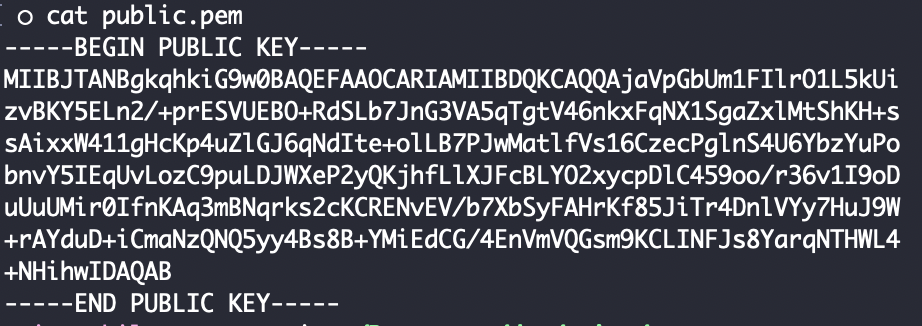
\includegraphics[scale=0.6]{publickey}
\caption{Clé publique que l'on souhaite casser}
\end{figure}
Nous allons extraire des informations sur la méthode de chiffrement: notamment le modulus et l'exponent. Le modulus est en fait la variable \(n\) et l'exponent \(e\).
Il ne nous manque plus qu'a trouver \(\phi(n) = (p - 1)(q - 1)\), donc essayer toutes les valeurs possibles de p et q. L'extraction des variables peut se faire grâce à openssl sur la clé publique. 
\begin{figure}[ht]
\centering
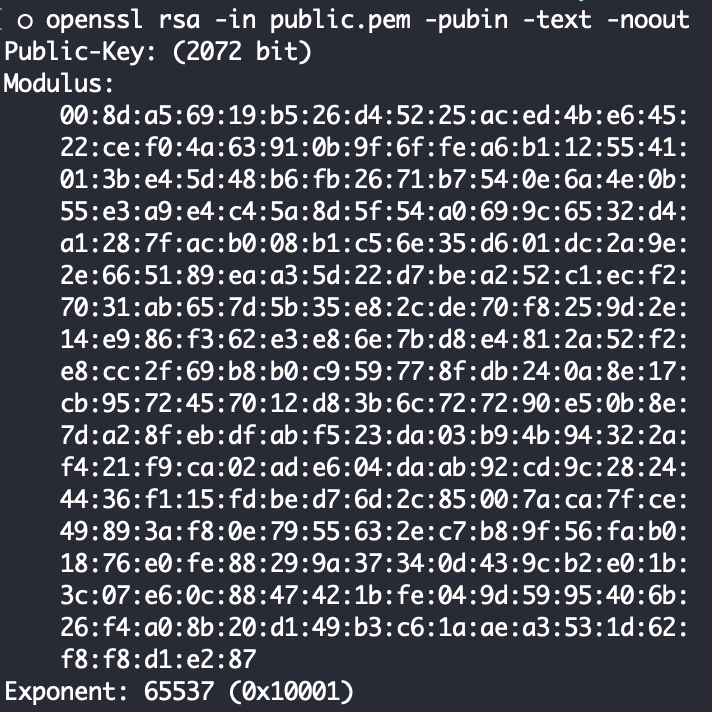
\includegraphics[scale=0.6]{modulus}
\caption{Extraction du modulus et de l'exponent}
\end{figure}
Nous savons que la génération de la clé a été faussée par le choix d'un \(p\) petit, il nous sera donc simple dans ce cas de factoriser, mais bien évidemment, dans un cas réel p et q seront tellement grands qu'il nous faudrait des décennies avant de pouvoir factoriser sur nos meilleurs ordinateurs. 
\begin{figure}[ht]
\centering
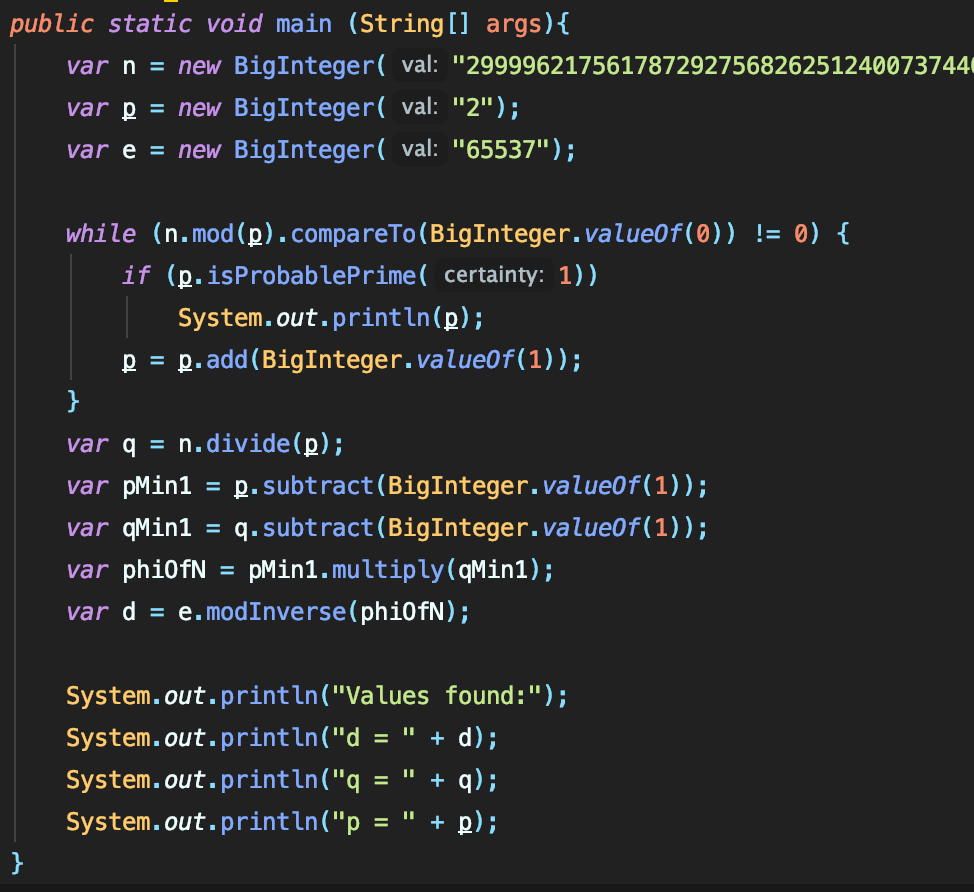
\includegraphics[scale=0.5]{algo}
\caption{Algorithme de factorisation}
\end{figure}

\section{Format ASN.1 DER}
Tout d'abord, créons un fichier private.txt contenant nos variables au format ASN.1: 
\begin{figure}[ht]
\centering
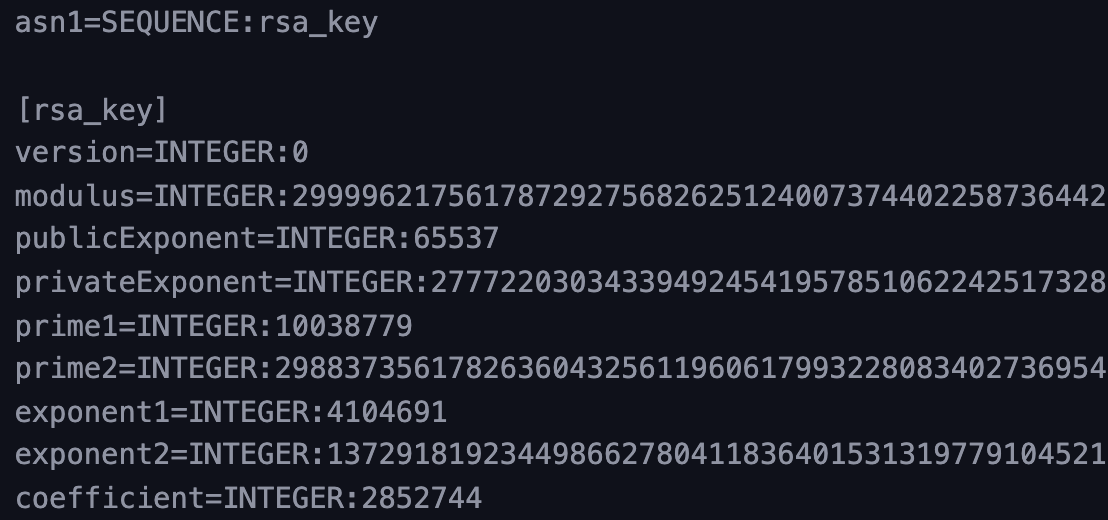
\includegraphics[scale=0.5]{der}
\caption{Clé RSA au format ASN.1}
\end{figure}
A partir de ce fichier private.txt, nous pouvons générer un fichier der:
\begin{verbatim}
openssl asn1parse -genconf private.txt -out private.der
\end{verbatim}

Puis vérifier que le certificat est valide en exportant toutes ces variables:
\begin{verbatim}
openssl rsa -in private.der -inform der -text -check
\end{verbatim}

Il nous est ensuite possible de reconstituer la clé privée avec:
\begin{verbatim}
openssl rsa -in private.der -inform der -out private_key.priv
\end{verbatim}

\section{Déchiffrement}

Grâce à cette clé privée, nous allons pouvoir déchiffrer la clé AES que nous avons:
\begin{figure}[ht]
\centering
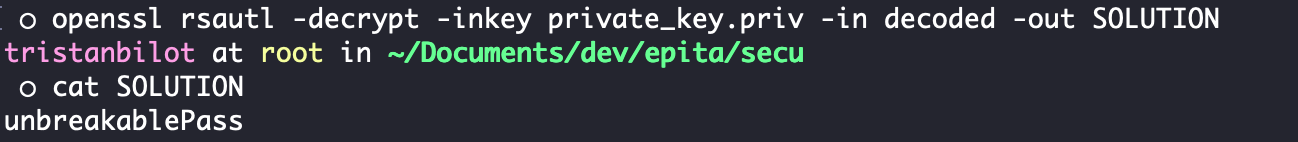
\includegraphics[scale=0.6]{aes_key}
\caption{Déchiffrement de la clé AES}
\end{figure}

Maintenant que la clé AES est en clair, il va être possible de l'utiliser pour déchiffrer le message originel. Il est important d'ajouter les mêmes paramètres de déchiffrement que ceux utilisés pour le chiffrement: c'est à dire aes-256-cbc sans sel.
\begin{figure}[ht]
\centering
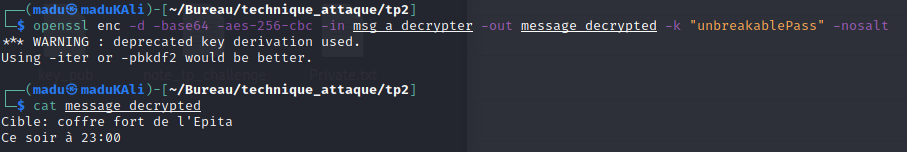
\includegraphics[scale=0.6]{answer}
\caption{Déchiffrement du message avec la clé AES}
\end{figure}
Le message est enfin déchiffré.

\end{document} 

